%%% Methods Section
\section{Methods}

In the case of the mono energic point source the source is directly surrounded by HDPE, as shown in Figure ~\ref{fig:PointSrcGeo}. 
The \iso[252]{Cf} source is not presented as a bare point source.
Rather, the source is modeled as as a point \iso[252]{Cf} source sournded by 0.5 cm of lead and 2.5 cm of HDPE in order to replicate the test source used for testing radiation portal monitors, as shown in Figure ~\ref{fig:Cf252SrcGeo}.
\begin{figure}
  \centering
  \begin{subfigure}[b]{0.45\textwidth}
    \centering
    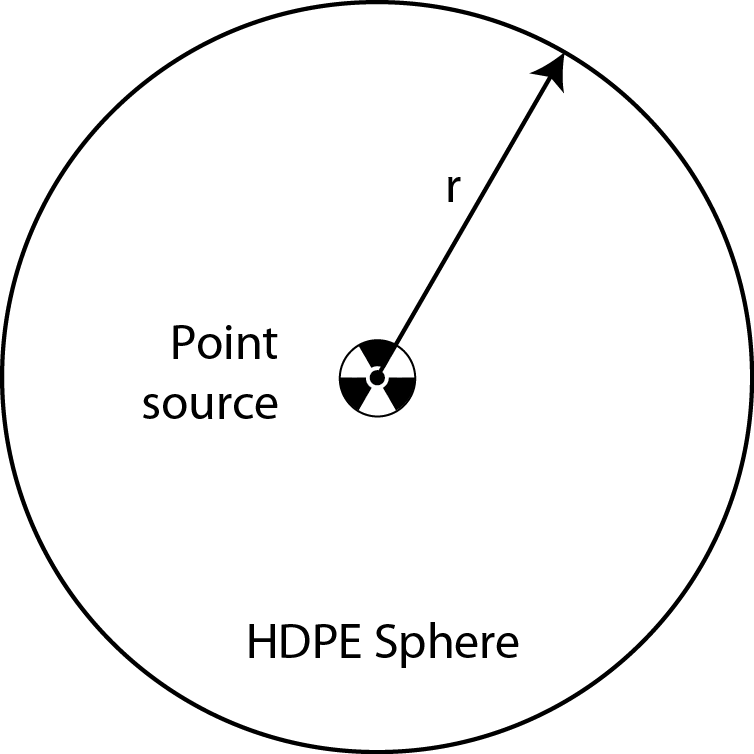
\includegraphics[width=\textwidth]{HDPEModeration_PointSrcGeo}
    \caption{Geometry of mono energetic point source}
    \label{fig:Cf252SrcGeo}
  \end{subfigure}%
  ~
  \begin{subfigure}[b]{0.45\textwidth}
    \centering
    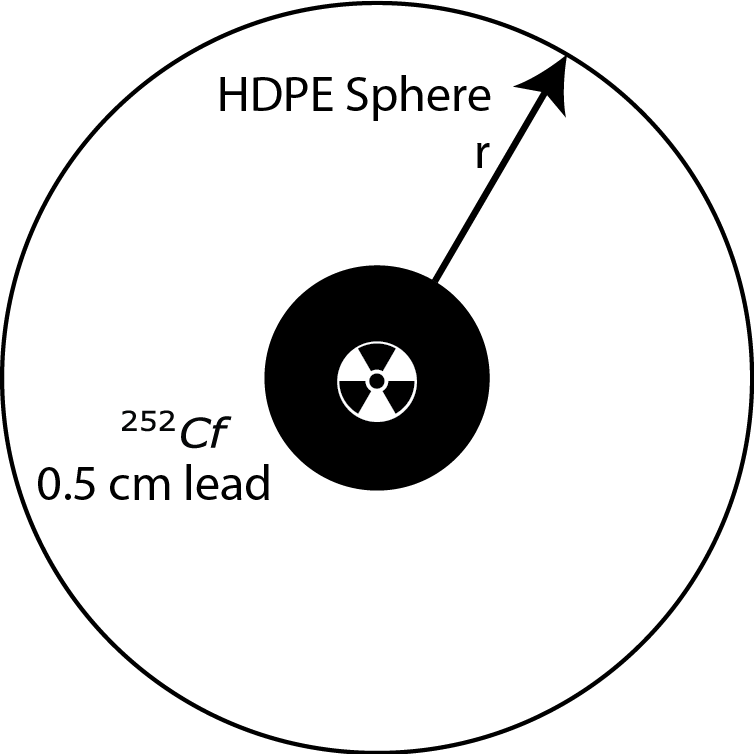
\includegraphics[width=\textwidth]{HDPEModeration_Cf252SrcGeo}
    \caption{Geometry of \isotope[252]{Cf} source}
    \label{fig:Cf252SrcGeo}
  \end{subfigure}
  \caption{Simulated Geometry}
\end{figure}
In both source configurations the source is so

\subsection{Simulation}
%%%%%%%%%%%%%%%%%%%%%%%%% LISTING CODE %%%%%%%%%%%%%%%%%%%%%%%%%%
%\lstinputlisting[linerange={217-220},caption=World Physical Volume,label=lst:World]{src/DetectorConstruction.cc}
